% 2010 年四川卷理科第 18 题：正方体 ABCD-A'B'C'D'，棱长 1，M 为 AA' 中点，O 为 BD' 中点。
% 来源 PDF：普通高考/2010/2010四川理.pdf，SHA-256 499425696359cfc2cf4418254bdaa1a37487b3dbaa072ff3c7cbe18dbabe73dc。
% 原页：第 1 页（A3 三栏）第 3 栏下部，书页码 631。
% 重绘依据：斜二测投影，竖棱竖直、深度方向斜向上；可见面为前面 ABB'A'、右面 BCC'B'、上面 A'B'C'D'；
%   被遮挡的 AD、DC、DD' 画虚线；MB、BC' 为面内连线（实线），BD'、MO、MC' 为体内连线（虚线）。
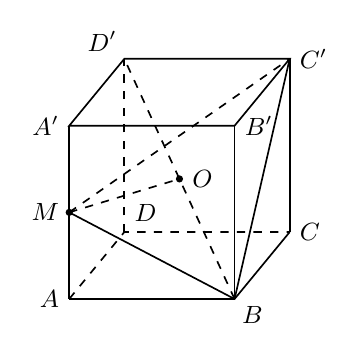
\begin{tikzpicture}[semithick, every node/.style={inner sep=1.4pt, font=\small}]
  \coordinate (A)  at (0.00,0.00);
  \coordinate (B)  at (2.10,0.00);
  \coordinate (C)  at (2.80,0.85);
  \coordinate (D)  at (0.70,0.85);
  \coordinate (A1) at (0.00,2.20);
  \coordinate (B1) at (2.10,2.20);
  \coordinate (C1) at (2.80,3.05);
  \coordinate (D1) at (0.70,3.05);
  \coordinate (M)  at (0.00,1.10);
  \coordinate (O)  at (1.40,1.525);

  % 可见棱
  \draw (A) -- (B) -- (C);
  \draw (C) -- (C1);
  \draw (B) -- (B1);
  \draw (A) -- (A1);
  \draw (A1) -- (B1) -- (C1) -- (D1) -- cycle;

  % 被遮挡的棱
  \draw[dashed] (A) -- (D) -- (C);
  \draw[dashed] (D) -- (D1);

  % 面内连线与体内连线
  \draw (M) -- (B);
  \draw (B) -- (C1);
  \draw[dashed] (B) -- (D1);
  \draw[dashed] (M) -- (O);
  \draw[dashed] (M) -- (C1);

  \fill (M) circle (1.3pt);
  \fill (O) circle (1.3pt);

  % 标注
  \node[left=2pt] at (A) {$A$};
  \node[below right=1pt] at (B) {$B$};
  \node[right=2pt] at (C) {$C$};
  \node[above right=2pt] at (D) {$D$};
  \node[left=2pt] at (A1) {$A'$};
  \node[right=2pt] at (B1) {$B'$};
  \node[right=2pt] at (C1) {$C'$};
  \node[above left=1pt] at (D1) {$D'$};
  \node[left=2pt] at (M) {$M$};
  \node[right=3pt] at (O) {$O$};
\end{tikzpicture}
